\documentclass{article}
\usepackage{pgfplots}
\begin{document}

\begin{figure}
    \centering
    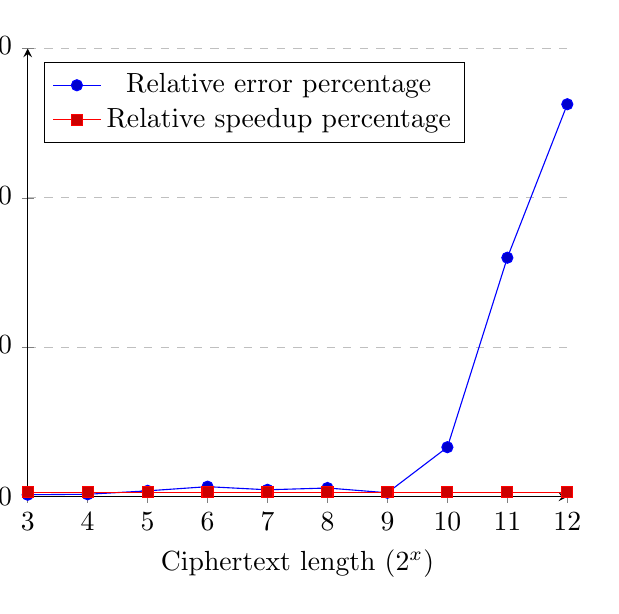
\begin{tikzpicture}[trim axis left]
        \begin{axis}[
            axis x line=bottom,
            axis y line=left,
            xlabel={Ciphertext length ($2^{x}$)},
            ylabel={Percentage},
            xmin=3,xmax=12,
            ymin=0,ymax=3000,
            legend pos=north west,
            xtick=data,
            ymajorgrids=true,
            grid style=dashed,
        ]
        \addplot coordinates {
            (3,14)(4,17)(5,40)(6,68)(7,47)(8,59)(9,27)(10,332)(11,1600)(12,2627)
        };
        \addlegendentry{Relative error percentage}
        \addplot coordinates {(3,30)(4,30)(5,30)(6,30)(7,30)(8,30)(9,30)(10,30)(11,30)(12,30)};
        \addlegendentry{Relative speedup percentage}
        \end{axis}
    \end{tikzpicture}
\end{figure}

\end{document}